\documentclass[titlepage]{article}

\usepackage[dutch]{babel}
\usepackage{fancyhdr}
\usepackage[margin=2cm]{geometry}
\usepackage{graphicx}
\usepackage[utf8]{inputenc}
\usepackage{siunitx}
\usepackage{tikz}

\usetikzlibrary{arrows}

\graphicspath{ {schermafdrukken/} }

\sisetup{detect-weight=true, detect-family=true}

\title{
    Practicum 2: \\
    \large{Een eenvoudige rekenmachine}
}

\author{
    Caro Meysmans \\
    \texttt{Caro.Meysmans@UGent.be}
    \and
    Lukas De Loose \\
    \texttt{Lukas.DeLoose@UGent.be}
    \and
    Garben Tanghe \\
    \texttt{Garben.Tanghe@UGent.be}
}

\pagestyle{fancy}

% Clear header and footer
\fancyhf{}

\lhead{Practicum 2}
\rhead{Een eenvoudige rekenmachine}
\lfoot{Groep 11}
\rfoot{Pagina \thepage}

\newcommand{\question}[1]{\noindent \textbf{#1} \\}

\begin{document}

\maketitle

\tableofcontents
\listoffigures

\clearpage

\section{Sequentiële modules in het datapad}

\subsection{De klok}

Onze implementatie maakt gebruik van de \SI{100}{\mega\hertz} klok die op de FPGA wordt gegenereerd.

\begin{figure}[h!]
    \centering

    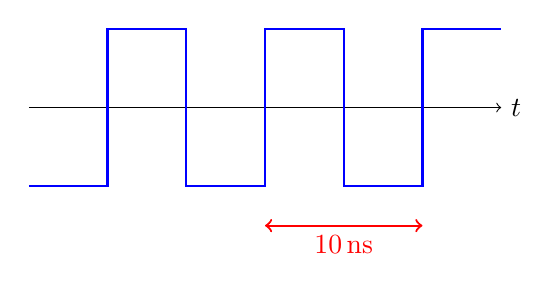
\begin{tikzpicture}[scale = 0.5]
        \draw[->] (-6, 0) -- (6, 0) node[right] { \( t \) };

        \draw[blue, thick] (-6, -2)
            -| (-4, 2)
            -| (-2, -2)
            -| (0, 2)
            -| (2, -2)
            -| (4, 2)
            -- (6, 2);

        \draw[<->, red, thick] (0, -3) -- (4, -3) node [midway, below] {\SI{10}{\nano\second}};
    \end{tikzpicture}

    \caption{Kloksignaal gegenereerd door de FPGA}
    \label{fig:kloksignaal}
\end{figure}

\subsection{De display driver}

\question{Hoe lang wordt elke individuele display aangestuurd bij een klokperiode van \SI{10}{\nano\second}?}
De display driver incrementeert \texttt{data\_selector} elke periode.
Dit signaal is 16 bits breed.
De 2 meest significante bits bepalen welke individuele display wordt aangestuurd.
Opdat deze veranderen, moeten we \( 2^{14} \) perioden doorstappen.
Dit betekent dat elke individuele display \SI{163.84}{\micro\second} wordt aangestuurd.

\subsection{Registers}

Het beschreven gedrag stelt dat het register asynchroon reageert op de \texttt{reset}-ingang en synchroon op de \texttt{enable}-ingang.
Dit wordt bevestigd door de onderstaande golfvormen.
In de gedragssimulatie bemerken we op \( t = \SI{5}{\nano\second} \) en \( t = \SI{70}{\nano\second} \) dat het \texttt{reset}-signaal asynchroon werkt.
Daarnaast merken we op \( t = \SI{25}{\nano\second} \) en \( t =\SI{35}{\nano\second} \) dat er correct wordt weggeschreven naar het register.
Op \( t = \SI{60}{\nano\second} \) wordt nogmaals bevestigd dat dit wegschrijven synchroon gebeurt.

\begin{figure}[h!]
    \centering
    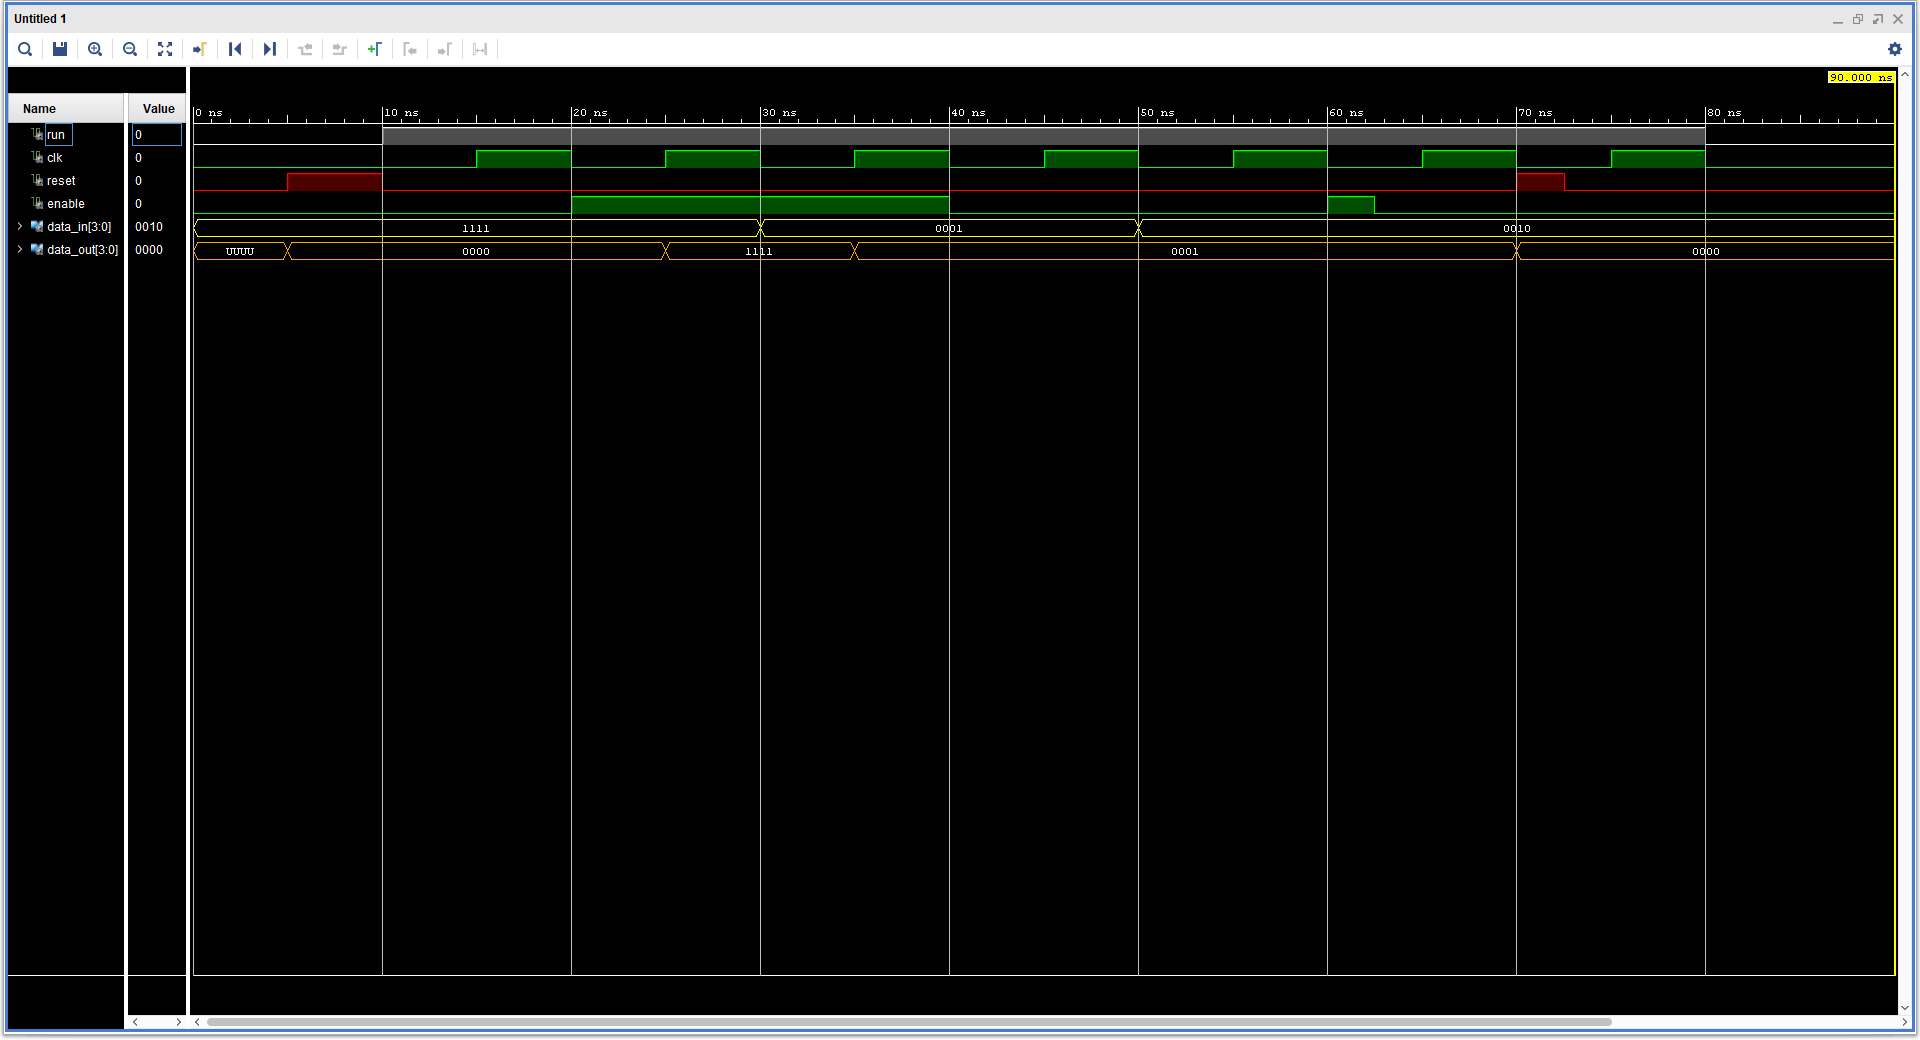
\includegraphics[trim={0 500px 0 0}, clip, width=0.8\linewidth]{Reg4_gedragssimulatie.PNG}
    \caption{\texttt{Reg4} gedragssimulatie}
    \label{fig:Reg4_gedragssimulatie}
\end{figure}

\clearpage

\subsection{Een synchrone BCD op- en neerteller}

Net als het register dient de BCD op- en neerteller een asynchrone \texttt{reset}-ingang en een synchrone \texttt{enable}-ingang te hebben.
In de gedragssimulatie bevestigt \( t = \SI{2.5}{\nano\second} \) de asynchrone werking van het resetsignaal.
Daarnaast stellen we tussen \( t = \SI{20}{\nano\second} \) en \( t = \SI{120}{\nano\second} \) een correcte optelling vast, wanneer de \texttt{direction}-ingang laag staat.
Tussen \( t = \SI{140}{\nano\second} \) en \( t = \SI{250}{\nano\second} \) gebeurt een correcte neertelling, wanneer de \texttt{direction}-ingang hoog staat.
Op \( t = \SI{115}{\nano\second} \) en \( t = \SI{245}{\nano\second} \) vindt de \textit{wraparound} plaats.
Tot slot zien we ook dat de data niet verandert wanneer de \texttt{enable}-ingang laag is.

\begin{figure}[h!]
    \centering
    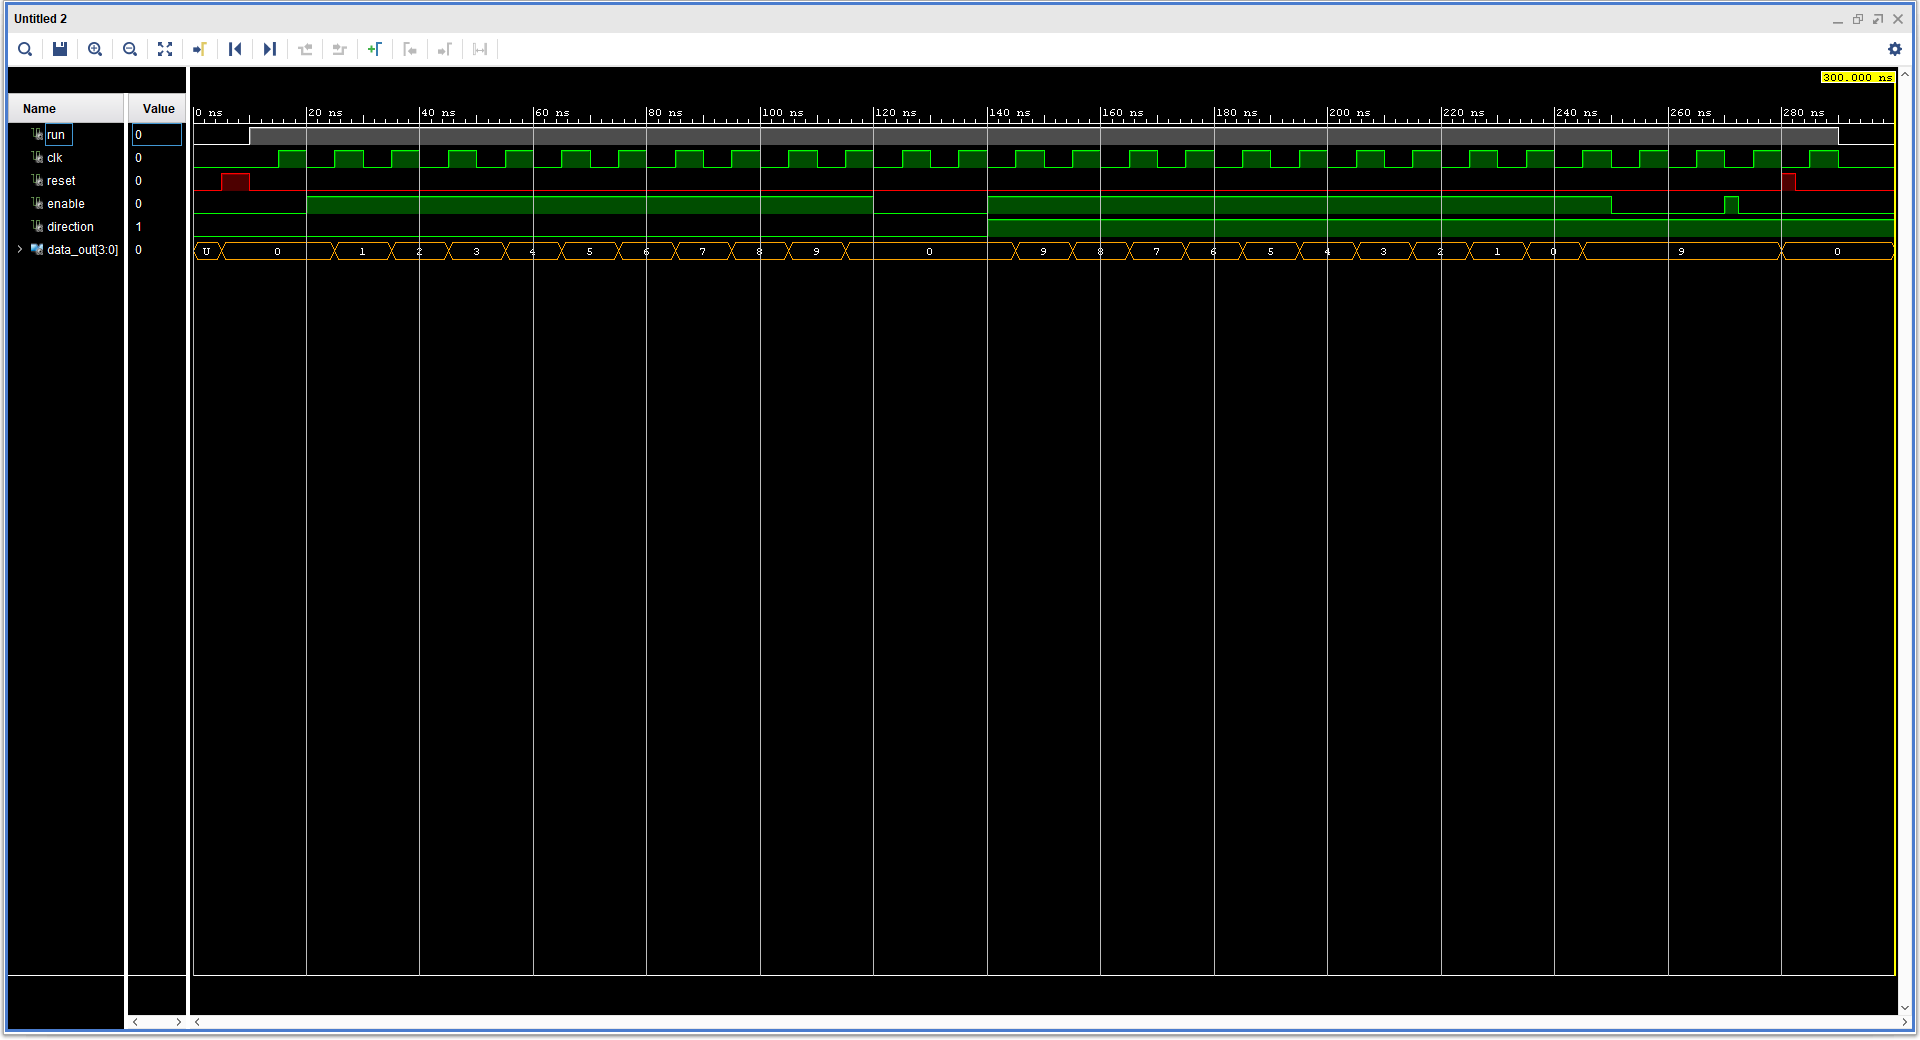
\includegraphics[trim={0 500px 0 0}, clip, width=0.8\linewidth]{bcd_counter_gedragssimulatie.PNG}
    \caption{\texttt{bcd\_counter} gedragssimulatie}
    \label{fig:bcd_counter_gedragssimulatie}
\end{figure}

Door vermoedelijk een bug in \textit{Vivado} bemerken we geen vertragingen in de post-implementatie tijdssimulatie.

\begin{figure}[h!]
    \centering
    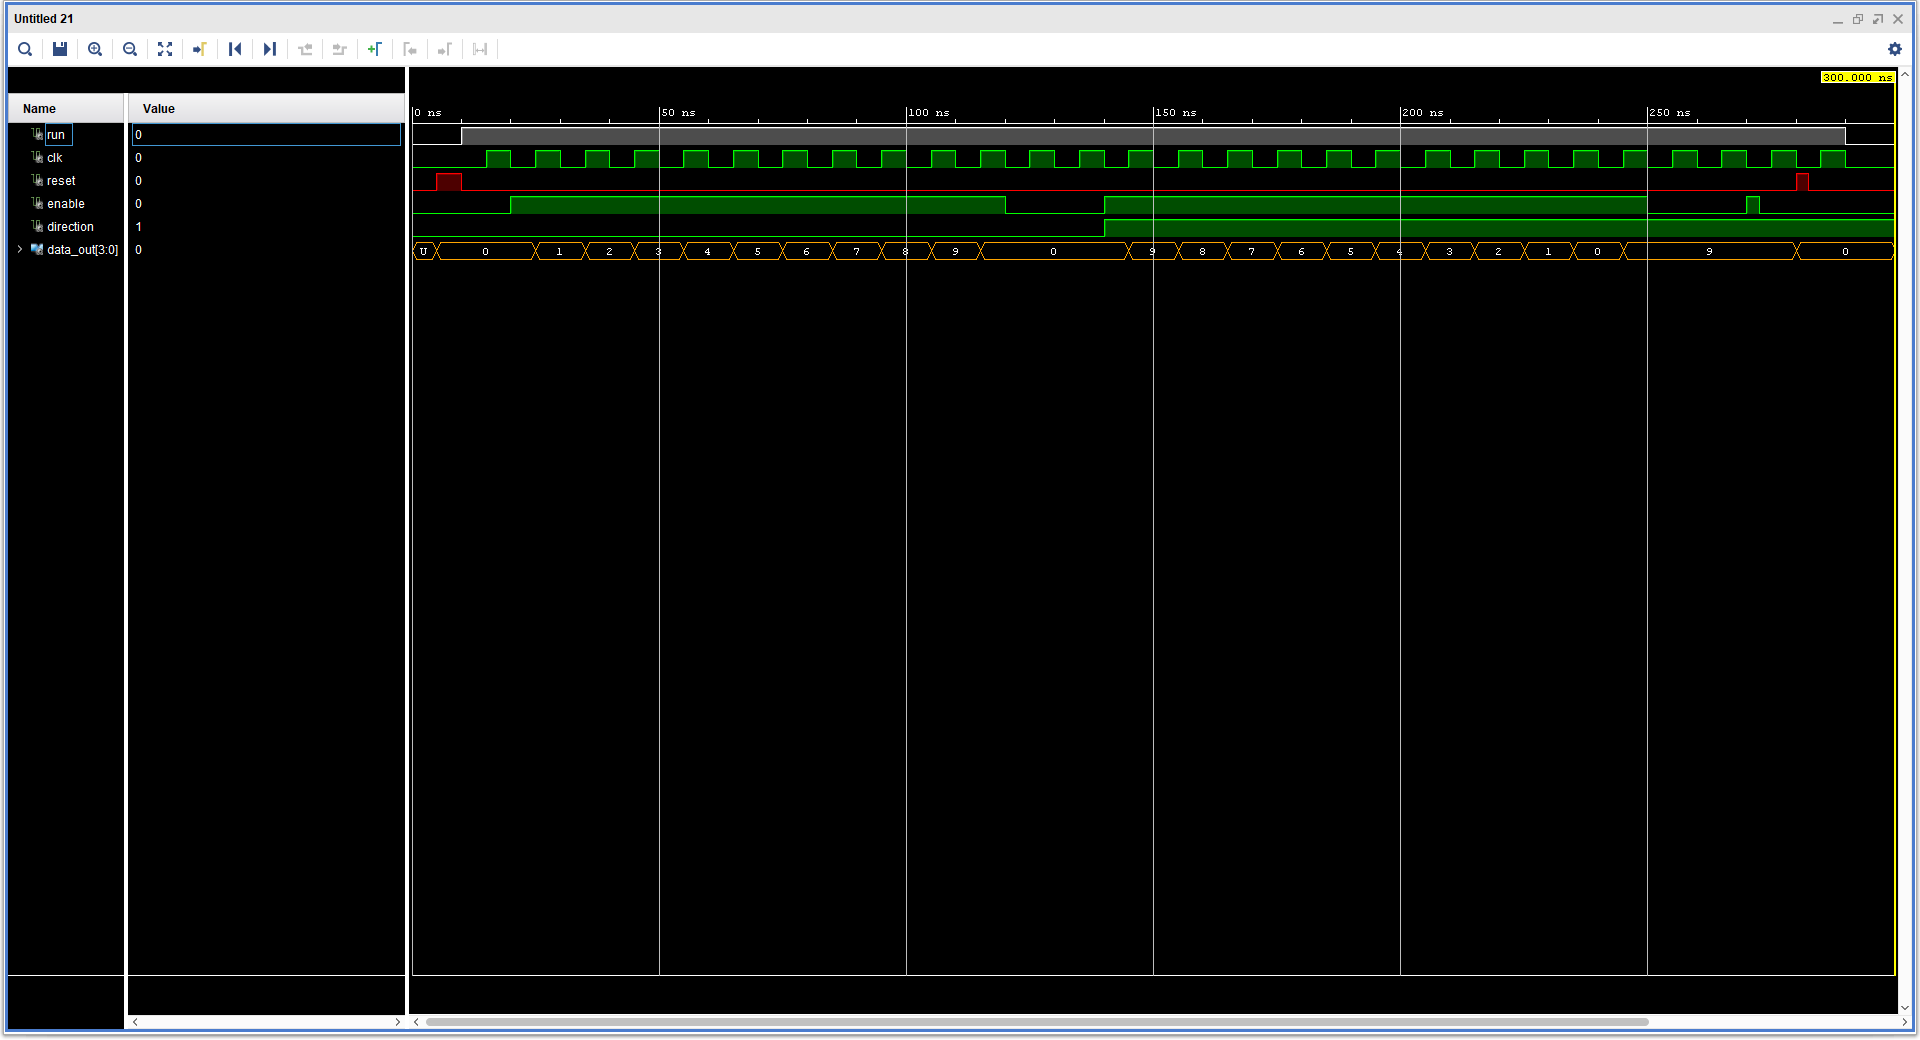
\includegraphics[trim={0 500px 0 0}, clip, width=0.8\linewidth]{bcd_counter_tijdssimulatie.PNG}
    \caption{\texttt{bcd\_counter} post-implementatie tijdssimulatie}
    \label{fig:bcd_counter_tijdssimulatie}
\end{figure}

\subsection{De knopjes}

Om het beschreven gedrag te realiseren dienen we ons te wenden tot een synchrone automaat met asynchrone \texttt{reset}-ingang en één uitgangsbit.
Het toestandstransitiediagram in figuur \ref{fig:button_pressed_toestandstransitiediagram} beschrijft de automaat in \texttt{button\_pressed}.
\( Y \) is de uitgangsbit.
De transitiecondities slaan op het al dan niet hoog zijn van de ingangsbit, het knopje.
De transitie van \texttt{state\_released} naar \texttt{state\_not\_pressed} is onvoorwaardelijk.
Wanneer \texttt{reset} hoog is, gaan we asynchroon terug naar de wachttoestand, \texttt{state\_wait}.

We bemerken dat bij een ingang die niet samenvalt met de klokflanken,
de uitgang alsnog één klokcyclus hoog blijft.

\begin{figure}[h!]
    \centering
    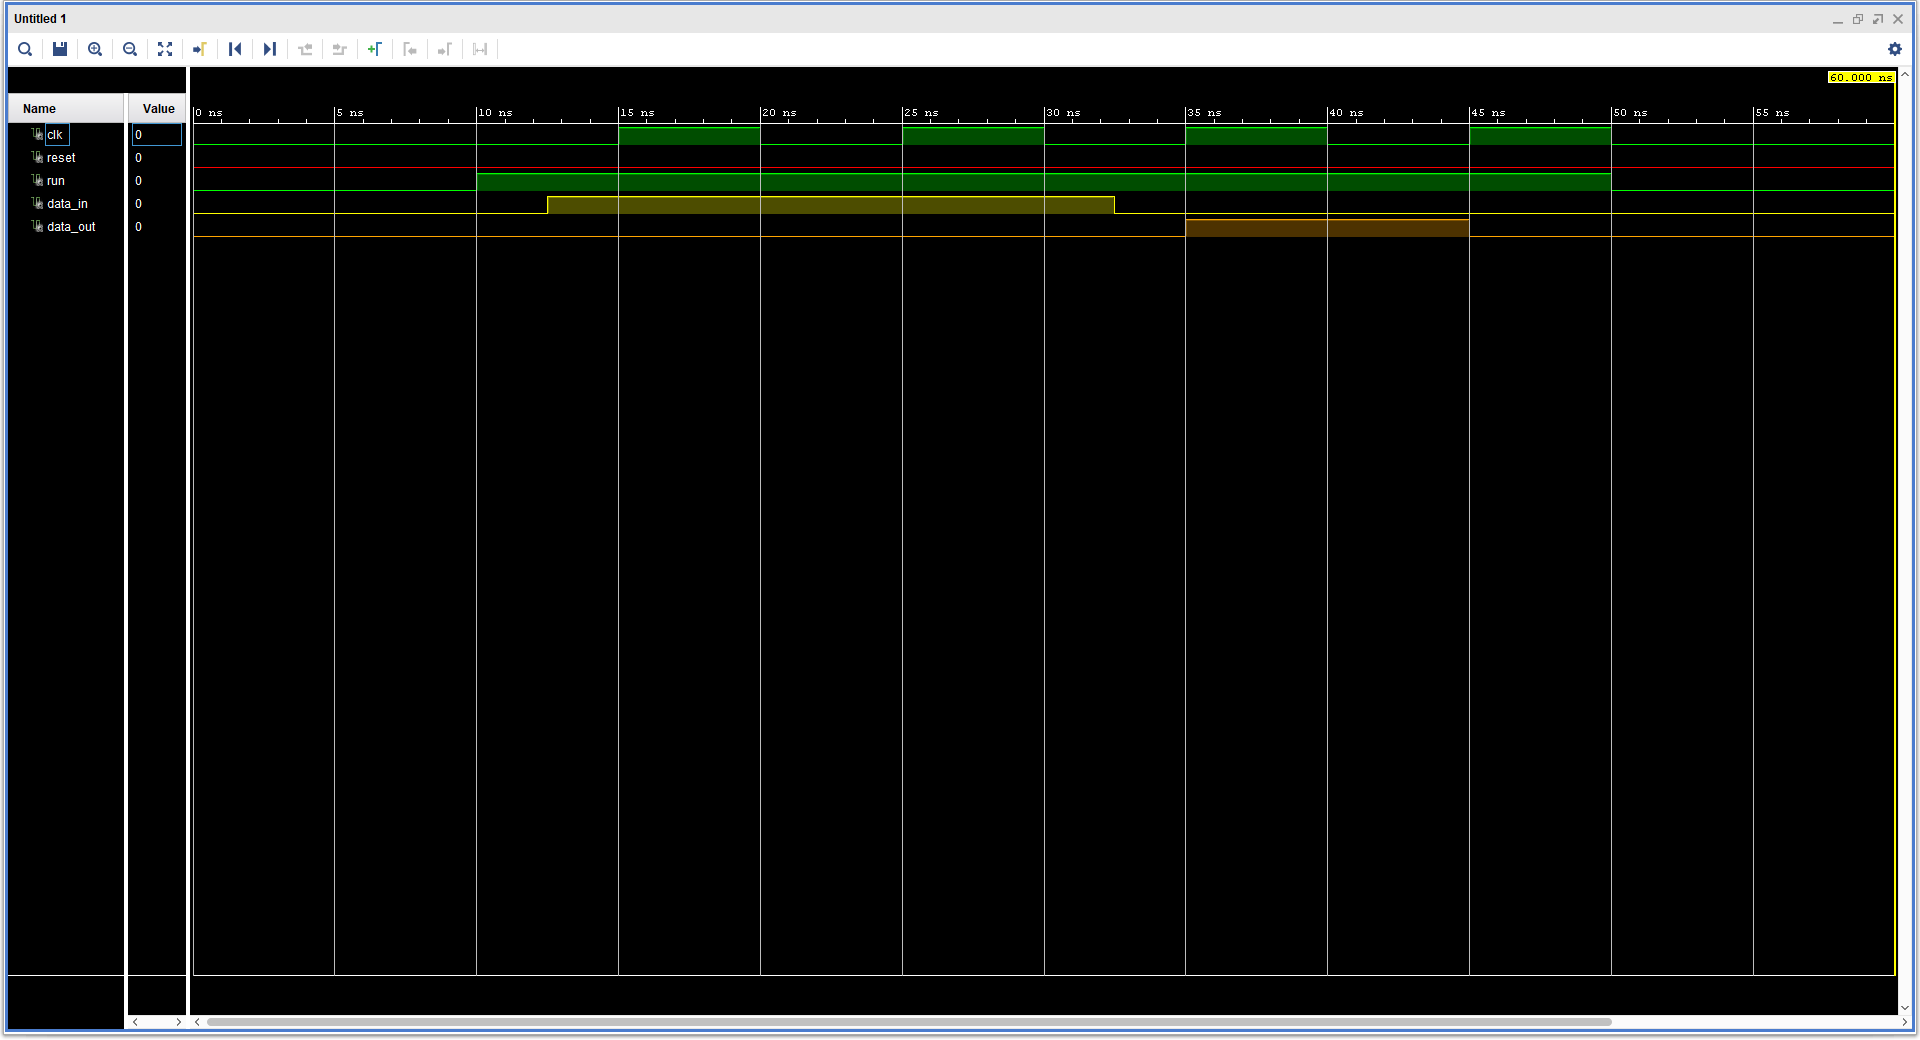
\includegraphics[trim={0 500px 0 0}, clip, width=0.8\linewidth]{button_pressed_gedragssimulatie.PNG}
    \caption{\texttt{button\_pressed} gedragssimulatie}
    \label{fig:button_pressed_gedragssimulatie}
\end{figure}

Door vermoedelijk een bug in \textit{Vivado} bemerken we geen vertragingen in de post-implementatie tijdssimulatie.

\begin{figure}[h!]
    \centering
    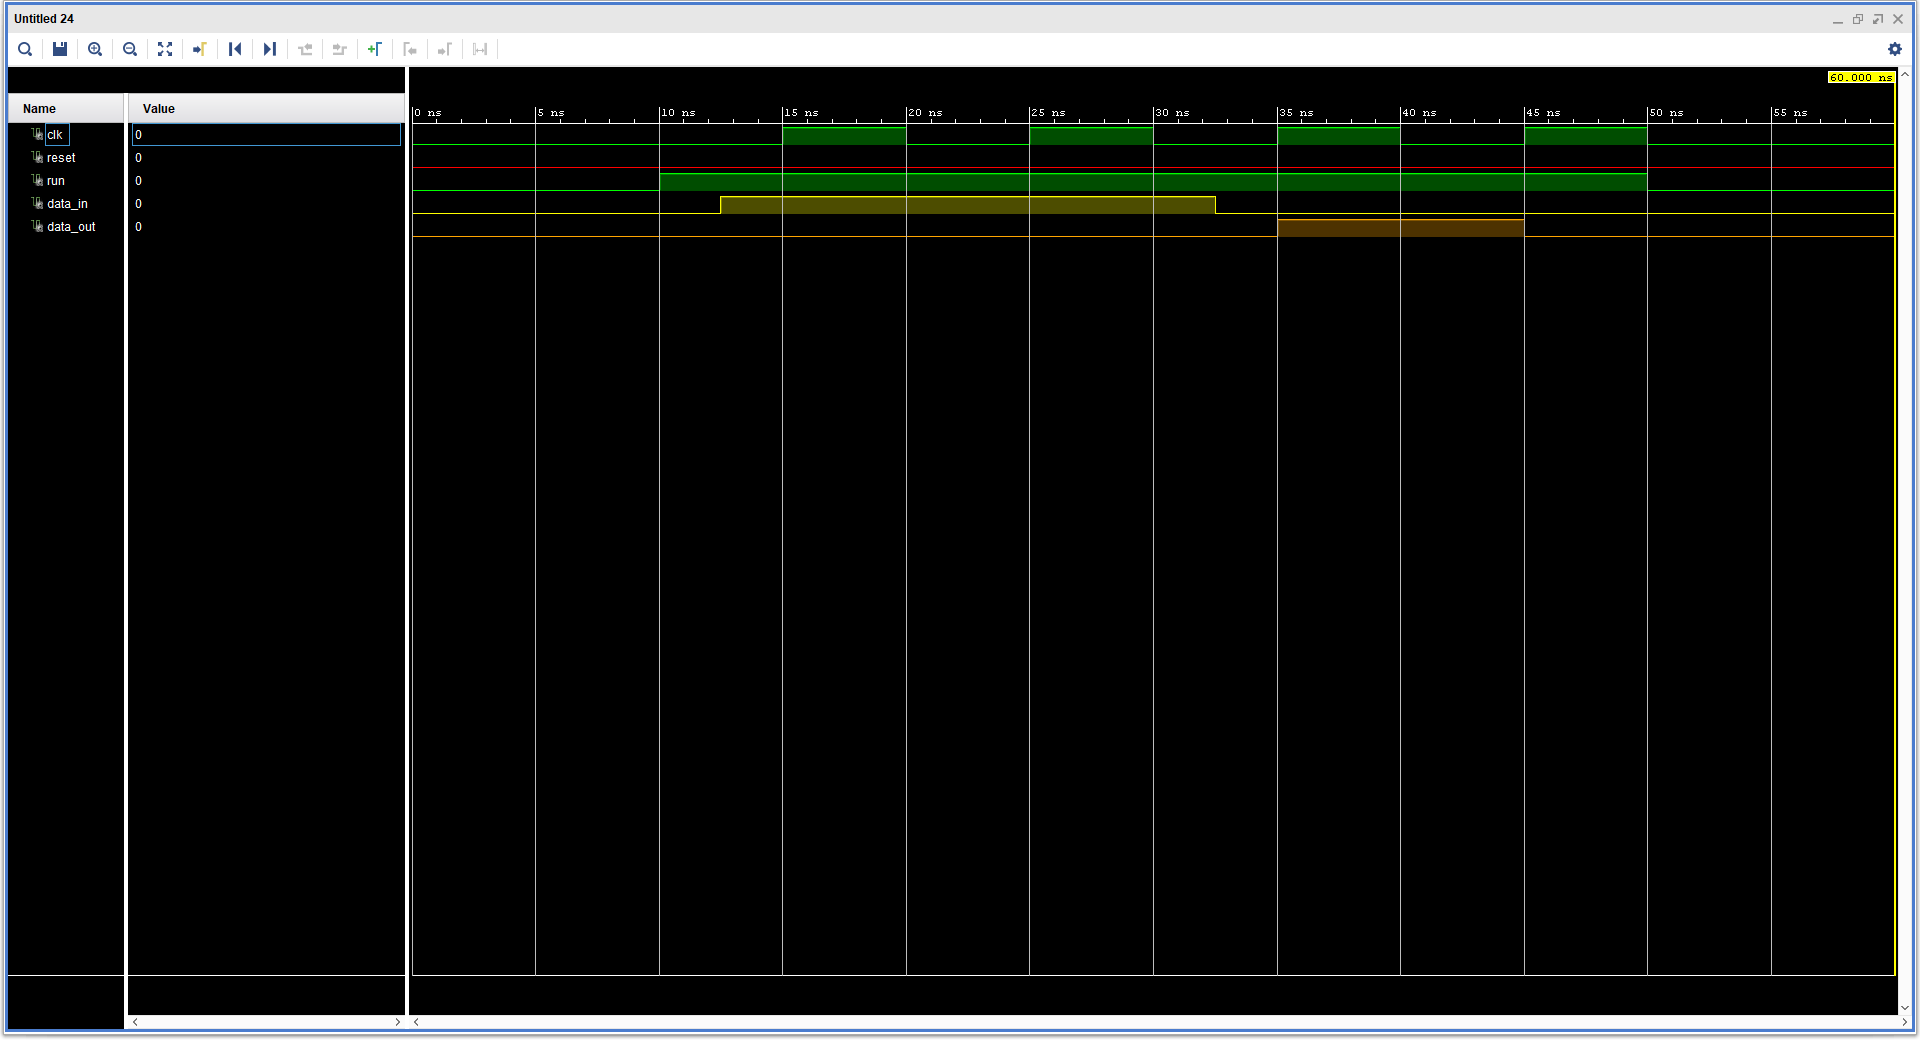
\includegraphics[trim={0 500px 0 0}, clip, width=0.8\linewidth]{button_pressed_tijdssimulatie.PNG}
    \caption{\texttt{button\_pressed} post-implementatie tijdssimulatie}
    \label{fig:button_pressed_tijdssimulatie}
\end{figure}

\begin{figure}[h!]
    \centering
    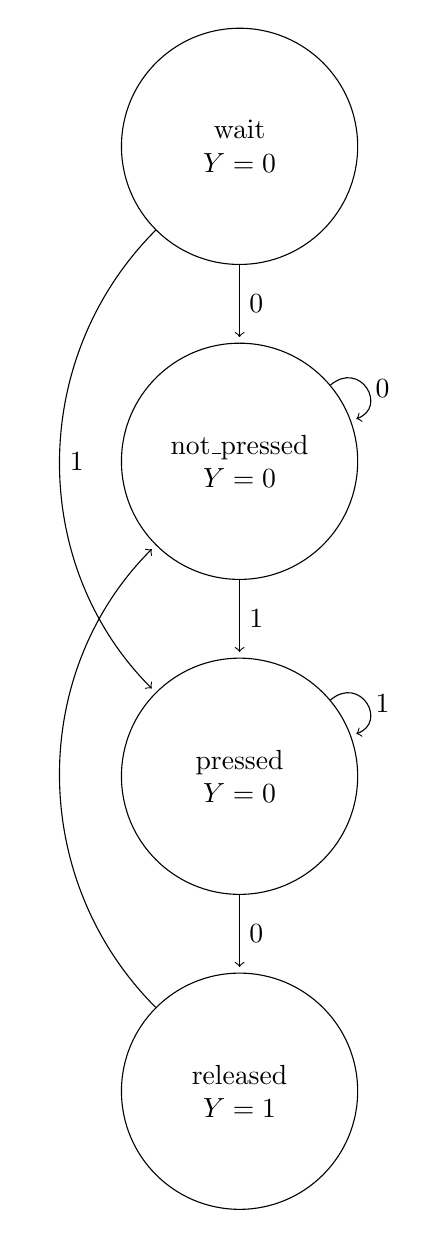
\begin{tikzpicture}[
            shorten >= 2 pt,
            state/.style = {
                draw, circle,
                align=center,
                minimum width = 3 cm,
                node distance = 4.0 cm,
            },
        ]

        % Toestanden
        \node[state] (wait) {wait \\ \(Y = 0\)};
        \node[state, below of = wait] (not_pressed) {not\_pressed \\ \(Y = 0\)};
        \node[state, below of = not_pressed] (pressed) {pressed \\ \(Y = 0 \)};
        \node[state, below of = pressed] (released) {released \\ \(Y = 1\)};

        % Transities
         \path
        [
            ->,
            every loop/.style = {
                in = 20,
                out = 40,
                looseness = 0
            }
        ]
            (not_pressed) edge[loop] node[right] {0} (not_pressed)
            (pressed) edge[loop] node[right] {1} (pressed);

        \path
        [
            ->
        ]
            (wait) edge node[right] {0} (not_pressed)
            (wait) edge[bend right = 45] node[right] {1} (pressed)
            (not_pressed) edge node[right] {1} (pressed)
            (pressed) edge node[right] {0} (released)
            (released) edge[bend left = 45] node {} (not_pressed);

    \end{tikzpicture}
    \caption{\texttt{button\_pressed} toestandstransitiediagram}
    \label{fig:button_pressed_toestandstransitiediagram}
\end{figure}

\newpage

\section{Het datapad en de controller}
<<<<<<< HEAD

\subsection{Het gedrag van de rekenmachine}

\subsection{Datapad en controller}

Het toestandsdiagram vindt u in figuur \ref{fig:rekenmachine_toestandstransitiediagram}.
Daarnaast vindt u ook een waarheidstabel van de uitgangen van de controller voor elke toestand in tabel \ref{tab:controlesignalen}.

\begin{figure}[h!]
    \centering

    \begin{tikzpicture}[
            shorten >= 2 pt,
            state/.style = {
                draw, circle,
                align=center,
                minimum width = 3 cm,
                node distance = 4.0 cm,
            },
        ]

        % Toestanden
        \node[state] (wait) {wait};
        \node[state, below of = wait] (operand_1) {operand\_1};
        \node[state, below of = operand_1] (operand_2) {operand\_2};
        \node[state, below of = operand_2] (operation) {operation};
        \node[state, below left of = operation] (result_subtract) {result\_subtract};
        \node[state, below right of = operation] (result_add) {result\_add};

        % Transities
        \path
        [
            ->,
            every loop/.style = {
                in = 20,
                out = 40,
                looseness = 0
            }
        ]
            (wait) edge[loop] node[right] {others} (wait)
            (operand_1) edge[loop] node[right] {others} (operand_1)
            (operand_2) edge[loop] node[right] {others} (operand_2)
            (operation) edge[loop] node[right] {others} (operation);

        \path
        [
            ->,
            every loop/.style = {
                in = -20,
                out = -40,
                looseness = 0
            }
        ]
            (result_add) edge[loop] node[right] {others} (result_add);

        \path
        [
            ->,
            every loop/.style ={
                in = 200,
                out = 220,
                looseness = 0
            }
        ]
            (result_subtract) edge[loop] node[left] {others} (result_subtract);

        \path[->]
            (wait) edge node[right] {button\_center} (operand_1)
            (operand_1) edge node[right] {button\_center} (operand_2)
            (operand_2) edge node[right] {button\_center} (operation);

        \path[->]
            (operation) edge[bend right = 20] node[left] {button\_left} (result_subtract)
            (operation) edge[bend left = 20] node[right] {button\_right} (result_add);

        \path[->]
            (result_subtract) edge[bend left = 60] node[left] {button\_center} (operand_1)
            (result_add) edge[bend right = 60] node[right] {button\_center} (operand_1);
    \end{tikzpicture}

    \caption{Toestandstransitiediagram}
    \label{fig:rekenmachine_toestandstransitiediagram}
\end{figure}

\begin{table}[h!]
    \centering

    \begin{tabular}{l|cccccc}
                            & operand\_1\_enable & operand\_2\_enable & operation & view\_output & view\_wait \\
        \hline
        wait                & 0                  & 0                  & 0         & 0            & 1 \\
        operand\_1          & 1                  & 0                  & 0         & 0            & 0 \\
        operand\_2          & 0                  & 1                  & 0         & 0            & 0 \\
        operation           & 0                  & 0                  & 0         & 0            & 0 \\
        result\_add         & 0                  & 0                  & 0         & 1            & 0 \\
        result\_subtract    & 0                  & 0                  & 1         & 1            & 0 \\
    \end{tabular}
    \caption{Controlesignalen}
    \label{tab:controlesignalen}
\end{table}

Onze controller genereert een aantal controlesignalen.
\texttt{operand\_1\_enable} en \texttt{operand\_2\_enable} laten toe de waarde van \texttt{counter}, de geselecteerde getalwaarde, door te schrijven naar de respectievelijke registers.
Daarnaast geeft \texttt{operation} aan welke bewerking de rekenmachine moet uitvoeren.
Indien dit signaal hoog staat, worden beide registers afgetrokken.
Een laag signaal impliceert daarentegen de optelling.
\texttt{view\_output} laat ons toe te selecteren wat er wordt doorgeschreven naar de schermpjes.
Een hoog signaal stuurt de uitgang van de \texttt{addsub4}-entiteit naar het schermpje.
Een laag signaal toont de waarde van de \texttt{operand}-ingang op het schermpje.
Als laatste hebben we \texttt{view\_wait}.
Deze laat toe bij een hoog signaal vier mintekens naar het scherm weg te schrijven.
Bij een laag signaal werkt \texttt{calculator} zoals hierboven beschreven.

We beginnen in een wachttoestand, \texttt{state\_wait}.
Hier staat de \texttt{view\_wait}-bit hoog, zodat er vier mintekens op het scherm worden geschreven.

Door op de centrale knop te drukken komen we in de toestand \texttt{state\_operand\_1}.
Deze toestand zorgt ervoor dat de \texttt{enable}-ingang van de teller hoog komt te staan.
Deze \texttt{enable}-ingang wordt namelijk berekend uit de \texttt{OF}-operatie van \texttt{operand\_1\_enable} en \texttt{operand\_2\_enable}.
Hierdoor kunnen we een eerste operand kunnen uitkiezen, daar \texttt{operand\_1\_enable} hoog staat, wordt deze ook weggeschreven naar het register van de eerste operand.
\texttt{state\_operand\_1} is op zich ook een automaat, maar werd hier vereenvoudigd tot één toestand.

De centrale knop indrukken brengt ons in de toesetand \texttt{state\_operand\_2}.
Deze is equivalent aan de vorige toestand, maar er wordt weggeschreven naar het register van de tweede operand.

Na weer op de centrale knop gedrukt te hebben komen we in de toestand \texttt{state\_operation}, waar we moeten kiezen of we optellen of aftrekken.

Indien we op de rechterknop drukken, komen we in de toestand \texttt{state\_result\_add}.
De \texttt{operation}-uitgang blijft laag, om aan te duiden dat we een optelling willen
De \texttt{view\_output}-bit wordt hoog gezet opdat we het resultaat naar het scherm wordt geprint.

Indien we op de linkerknop drukken, komen we in de toestand \texttt{state\_result\_subtract},
waar gelijkaardig aan de optelling de \texttt{view\_output}-bit hoog wordt gezet.
Wat wel verschilt, is de \texttt{operation}-bit.
Diens hoge toestand duidt op een aftrekking.

In beide situaties komen we na het drukken op de centrale knop weer in de toestand \texttt{state\_operand\_1}, waarna het verhaal herbegint.


Het blokschema kan u vinden in \texttt{bijlagen/blokschema.pdf}.
In wat volgt zullen we met oog op dit schema de implementatie van het datapad bespreken.

De uitgang van de BCD op- en neerteller, \texttt{operand}, wordt aangelegd aan twee registers.
Deze hebben als \texttt{enable}-signaal respectievelijk \texttt{operand\_1\_enable} en \texttt{operand\_2\_enable} en als uitgangen \texttt{operand\_1} en \texttt{operand\_2}.
Het signaal \texttt{operation} geeft aan of we optellen of aftrekken.

Het teken van het resultaat wordt als selectiebit aangelegd aan een twee-naar-één-multiplexer, met als ingangen \texttt{"0000"} en \texttt{"1111"}.
Bij een negatief teken wordt de uitgang \texttt{"1111"}. Een positief teken levert de uitgang \texttt{"0000"}.
De uitgang, \texttt{internal\_display\_data\_3}, representeert de derde nibble van \texttt{display\_data}.
Dit schrijft het eventuele minteken weg naar het scherm.

Daarnaast inverteren we de \texttt{sign}-bit en voeren we de \texttt{EN}-operatie uit met de \texttt{carry}-bit.
Indien het resultaat negatief kunnen we namelijk geen getallen kleiner dan \(-9\) wegschrijven.
Vervolgens concateneren we dit met het resultaat van de optelling.
Dit 5-bit getal wordt vervolgens aangelegd aan een multiplexer.
De andere ingang van de multiplexer is de \texttt{operand}-ingang.
Als selectiebit wordt \texttt{view\_output} gebruikt.
De betekenis hiervan werd reeds in de vorige paragraaf uitgelegd.

Dit resultaat wordt vervolgens gedecodeerd.
Dit levert twee 4-bit signalen, de twee decimalen van het resultaat, \texttt{internal\_display\_data\_2} en \texttt{internal\_display\_data\_1}.

Het schermpje verwacht een 16-bit getal.
Dit bekomen we door de bitsequentie \texttt{"0000"}, de lege eerste display, en de overige \texttt{internal\_display\_data}-signalen te concateneren.

Dit resultaat wordt aangelegd aan een twee-naar-één multiplexer.
De andere ingang is het signaal \texttt{"0xFFFF"}, vier mintekens.
Hiertussen kan geselecteerd worden door \texttt{view\_wait}.

Vervolgens bekomen we en 16-bit getal, klaar om weggeschreven te worden door de \texttt{multiple\_display\_driver}.

De \texttt{display\_mask} wordt geselecteerd door \texttt{view\_wait}.
Een hoge waarde levert \texttt{"1111"}.
Bij een lage waarde bekomen we een concatenatie van \texttt{'0'},
de vierde display is nooit aan,
de \texttt{EN}-operatie van \texttt{view\_output} en \texttt{add\_subtract\_sign},
we willen slechts een teken tonen, wanneer het resultaat wordt getoond en er daardwerkelijk een teken aanwezig is,
\texttt{internal\_display\_data\_2(0)},
het aanwezig zijn van een tiental, en \texttt{'1'}.


\subsection{Verificatie met ROM-bestanden}

\begin{figure}[h!]
    \centering
    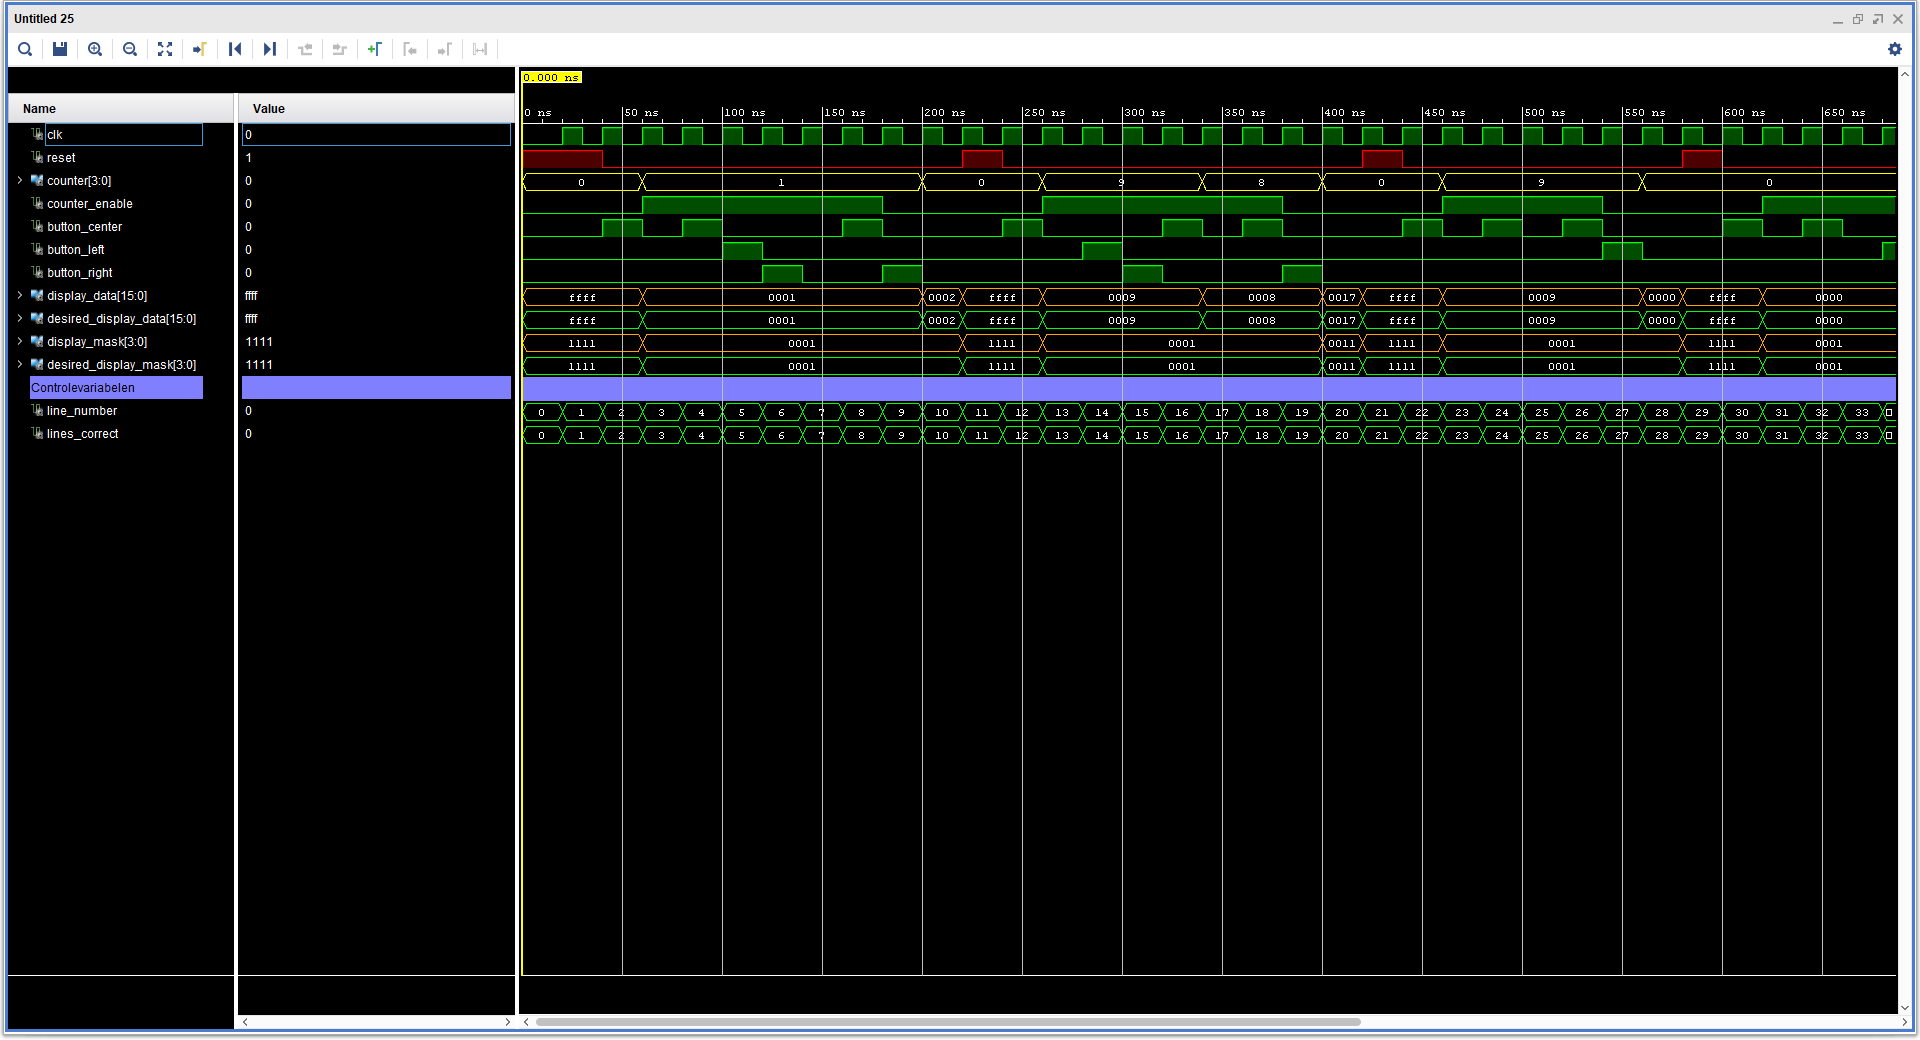
\includegraphics[trim={0 400px 0 0}, clip, width=0.8\linewidth]{calculator_gedragssimulatie.PNG}
    \caption{\texttt{calculator} gedragssimulatie}
    \label{fig:calculator_gedragssimulatie}
\end{figure}

Om het \texttt{.mem}-bestand te genereren,
hebben we een \textit{Python}-script geschreven.
De broncode is terug te vinden in \texttt{GenerateCalculatorMemory.py}.

\subsection{Testen in hardware}

Nadat we overtuigd waren dat het gedrag in hardware voldeed aan het beschreven gedrag,
lieten we onze finale realisatie evalueren door de professor.
Deze garandeerde ons de correcte werking.

\end{document}

